\documentclass{beamer}
    \usepackage{tikz}  %preable序言
    \usepackage{graphicx}
    \usepackage{color}
    % \usepackage{tikz}
    \usepackage{pgfplots}
    \usepackage{pgf-umlsd}
    \usepackage{ifthen}
    
\begin{document}
    \begin{frame}
        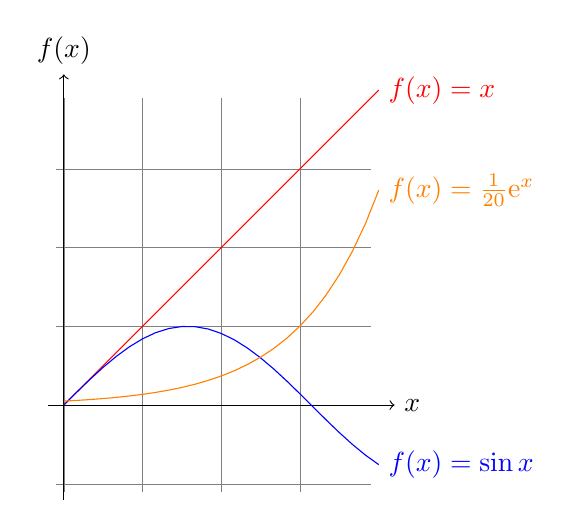
\begin{tikzpicture}[domain=0:4]
            \draw[very thin,color=gray] (-0.1,-1.1) grid (3.9,3.9);
            \draw[->] (-0.2,0) -- (4.2,0) node[right] {$x$};
            \draw[->] (0,-1.2) -- (0,4.2) node[above] {$f(x)$};
            \draw[color=red]    plot (\x,\x)             node[right] {$f(x) =x$};
            % \x r 表示弧度
            \draw[color=blue]   plot (\x,{sin(\x r)})    node[right] {$f(x) = \sin x$};
            \draw[color=orange] plot (\x,{0.05*exp(\x)}) node[right] {$f(x) = \frac{1}{20} \mathrm e^x$};
          \end{tikzpicture}
    \end{frame}

    \begin{frame}
        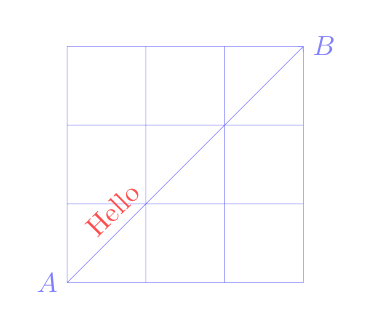
\begin{tikzpicture}
            \draw[help lines](0,0)grid(3,3) [color=blue!50,->](0,0) node[left]{$A$}-- node [color=red!70,pos=0.25,
                    above,sloped]{Hello}(3,3) node[right]{$B$};
        \end{tikzpicture}
    \end{frame}
% \begin{tikzpicture}
%     \node[anchor=south west,inner sep=0] (image) at (0,0) {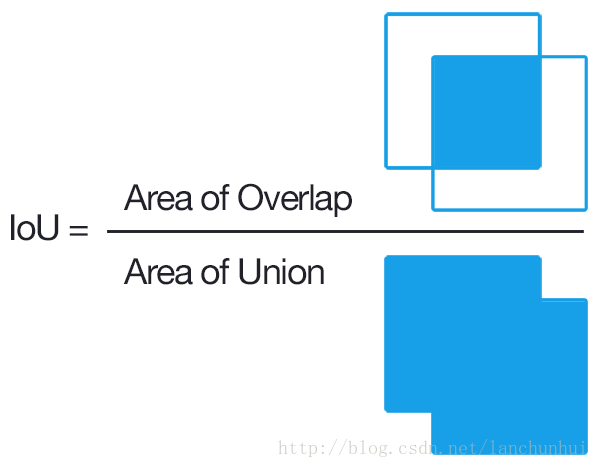
\includegraphics[width=0.9\textwidth]{../graphic/iou.png}};
%     \begin{scope}[x={(image.south east)},y={(image.north west)}]
%         \draw[red,ultra thick,rounded corners] (0.62,0.65) rectangle (0.78,0.75);
%     \end{scope}
% \end{tikzpicture}
% \end{document}
    \begin{frame}
        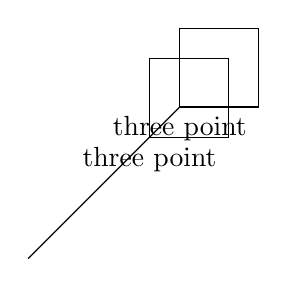
\begin{tikzpicture}
            \draw (0,0,0)--(0,0,5);
            \draw (0,0,0) -- (1,0,0) -- (1,1,0) -- (0,1,0) -- (0,0,0) node [below] {three point};
            \draw (0,0,1) -- (1,0,1) -- (1,1,1) -- (0,1,1) -- (0,0,1) node [below] {three point};
        \end{tikzpicture}
    \end{frame}

    \begin{frame}
        \begin{tikzpicture}
            \draw[->] (0,0,0) -- (5,0,0) node[right] {x};
            \draw[->] (0,0,0) -- (0,5,0) node[right] {y};
            \draw[->] (0,0,0) -- (0,0,5) node[right] {z};
        \end{tikzpicture}
    \end{frame}

    \begin{frame}
        
\begin{tikzpicture}
            % \newcommand\tikzmark[1]{%
            %     \tikz[overlay,remember picture] \node[coordinate] (#1) {};%
            % }
            \newcommand{\tikzmark}[1]{
                \node[coordinate]  {};
            }

            % \tikzmark{b}
            % \draw[->] (0,0,0) -- (5,0,0) node[right] {x};
            % \draw[->] (0,0,0) -- (0,5,0) node[right] {y};
            % \draw[->] (0,0,0) -- (0,0,5) node[right] {z};
            % \draw[->] (a) .... (b);            sdfsd
            \node[right] at (0,0) {$this is tikz corrd$};
        \end{tikzpicture}
    \end{frame}


\end{document}